\documentclass[a4paper,11pt]{article}
\usepackage[utf8]{inputenc}
\usepackage{amsmath}
\usepackage{amsfonts}
\usepackage{amssymb}
\usepackage{graphicx}
\usepackage{braket}

\numberwithin{equation}{section}
\renewcommand\thesubsection{\alph{subsection}}
\newcommand{\bvp}[1]{\mathbf{#1}'}
\newcommand{\bv}[1]{\mathbf{#1}}
\newcommand{\ez}{\epsilon_0}
\newcommand{\eo}{\epsilon_1}
\newcommand{\lrp}[1]{\left({#1}\right)}
\newcommand{\lrb}[1]{\left\{{#1}\right\}}


%opening
\title{Electromagnetic Theory II HW6}
\author{Vince Baker}

\begin{document}

\maketitle

\section*{8.4}
The general wave equation for a cylindrical waveguide is:
\begin{align}
 \lrp{\nabla_t^2+\gamma^2}\psi &= 0\\
 \psi &= E_z\textbf{ (TM) ,}B_z\textbf{ (TE)}
\end{align}
The solutions that are regular at $\rho=0$ are:
\begin{align}
 \psi &= A_m J_m(\gamma\rho)e^{\pm im\phi}
\end{align}
The boundary conditions on the conductor surface $\rho=R$ will be different for TE and TM modes.
For TM modes the E field vanishes at the surface, so the eigenvalues are the zeros of $J_m(\gamma R)$.
For TE modes the normal derivative of the magnetic field vanishes at the surface, so the eigenvalues are the zeros of $J'_m(\gamma R)$.
Therefore the mode frequencies are:
\begin{align}
 \omega_{m,n} &= \frac{Z_m(n)}{\sqrt{\mu\epsilon}R}\textbf{ (TM)}\\
 \omega_{m,n} &= \frac{Z'_m(n)}{\sqrt{\mu\epsilon}R}\textbf{ (TE)}
\end{align}
Where we have defined $Z_m(n)$ as the Nth zero of $J_m$ and $Z'_m(n)$ as the Nth zero of $J'_m$. 
The first few roots are:
\begin{align}
 Z_0 &= 2.41, 5.52, 8.65\\
 Z_1 &= 3.83, 7.02, 10.17\\
 Z_2 &= 5.14, 8.41, 11.62\\
 Z'_0 &= 3.83, 7.02, 10.17\\
 Z'_1 &= 1.84, 5.33, 8.54\\
 Z'_2 &= 3.05, 6.71, 9.97
\end{align}
The lowest root is $Z'_1(1)$, so the the dominant mode is $TE_{11}$. 
Listing the dominant mode and the next four higher modes:
\begin{tabular}{l | c | r}
 Mode & Frequency & Ratio\\
 \hline
 $TE_{11}$ & 1.84  & 1\\
 $TM_{01}$ & 2.41  & 1.31 \\
 $TE_{21}$ & 3.05 & 1.66\\
 $TE_{01},TM_{11}$ & 3.83 & 2.08\\
 $TM_{21}$ & 5.14 & 2.79
\end{tabular}
\\ \\
b) The attenuation coefficients are found from (Jackson 8.57):
\begin{align}
 \beta_\lambda &= -\frac{1}{2P}\frac{dP}{dz}
\end{align}
The power and power loss for TE and TM modes are:
\begin{align}
 P_{TM} &= \frac{1}{2\sqrt{\mu\epsilon}}\lrp{\frac{\omega}{\omega_\lambda}}^2 \lrp{1-\frac{\omega_\lambda^2}{\omega^2}}^{1/2}\epsilon \int_A \psi^* \psi\ da\\
 \frac{dP}{dz}_{TM} &= \frac{1}{2\sigma\delta}\lrp{\frac{\omega}{\omega_\lambda}}^2\oint_C \frac{1}{\mu^2\omega_\lambda^2}|\frac{\partial \psi}{\partial n}|^2\ d\ell\\
 P_{TE} &= \frac{1}{2\sqrt{\mu\epsilon}}\lrp{\frac{\omega}{\omega_\lambda}}^2 \lrp{1-\frac{\omega_\lambda^2}{\omega^2}}^{1/2}\mu \int_A \psi^* \psi\ da\\
 \frac{dP}{dz}_{TE} &= \frac{1}{2\sigma\delta}\lrp{\frac{\omega}{\omega_\lambda}}^2
	      \oint_C \frac{1}{\mu\epsilon\omega_\lambda^2}\lrp{1-\frac{\omega_\lambda^2}{\omega^2}}|\bv{n}\times\nabla_t\psi|^2 
	      +|\frac{\partial \psi}{\partial n}|^2\ d\ell
\end{align}
We can evaluate the power expressions for the TM modes using the orthogonality of the Bessel functions:
\begin{align}
 \int_0^1 xJ_m\lrp{xZ_m(n)}J_m\lrp{xZ_m(n)}\ dx &= \frac{1}{2}\left[J_{m+1}\lrp{xZ_m(n)}\right]^2
\end{align}
For the TM modes, integrating from $\rho=0$ to $R$ with $u \equiv Z_m(n)/R$ making the substitution $\rho' = \rho/R$ we find:
\begin{align}
 P_{TM} &= \frac{1}{2}\sqrt{\frac{\epsilon}{\mu}}\lrp{\frac{\omega}{\omega_\lambda}}^2\lrp{1-\frac{\omega_\lambda^2}{\omega^2}}^{1/2} 2\pi\int_0^1R^2\rho' \left[ J_m(\rho' Z_m(n))\right]^2\ d\rho'\\
 P_{TM} &= \frac{1}{2}\sqrt{\frac{\epsilon}{\mu}}\lrp{\frac{\omega}{\omega_\lambda}}^2\lrp{1-\frac{\omega_\lambda^2}{\omega^2}}^{1/2}\pi R^2\left[J_{m+1}(Z_m(n))\right]^2
\end{align}
The normal derivative is just $-\frac{d\psi}{d\rho}$, so we can calculate the power loss:
\begin{align}
 \frac{d\psi}{d\rho} &= -\gamma J'_m\lrp{Z_m(n)}e^{im\phi}\\
 \frac{dP}{dz} &= -\frac{1}{2\sigma\delta}\frac{\epsilon}{\mu}(2\pi R)[J'_m(Z_m(n))]^2\\
 \frac{dP}{dz} &= -\frac{1}{2\sigma\delta}\frac{\epsilon}{\mu}(2\pi R)[J_{m+1}(Z_m(n))]^2
\end{align}
Where in the last step we have used a recursion relation for Bessel functions.
We can now calculate the attenuation coefficient:
\begin{align}
 \beta_\lambda &= \frac{1}{2\sigma\delta}\lrp{\frac{\epsilon}{\mu}}^{3/2}\lrp{1-\frac{\omega_\lambda^2}{\omega^2}}^{1/2}\frac{2\pi R}{\pi R^2}\\
 \beta_\lambda &= \frac{1}{\sigma\delta}\lrp{\frac{\epsilon}{\mu}}^{3/2}\lrp{1-\frac{\omega_\lambda^2}{\omega^2}}^{1/2}\frac{1}{R}
\end{align}
\\
For the TE modes we are working with the zeros of the derivatives of the Bessel functions. 
Using an identity:
\begin{align}
 \int_0^1 x\left[J_m(ax) \right]^2\ dx &= \frac{1}{2}\lrp{[J'_m(a)]^2+(1-m^2/a^2)[J_m(a)]^2}
\end{align}
We calculate the power in the TE modes:
\begin{align}
 P_{TE} &= \frac{1}{2}\sqrt{\frac{\mu}{\epsilon}}\lrp{\frac{\omega}{\omega_\lambda}}^2\lrp{1-\frac{\omega_\lambda^2}{\omega^2}}^{1/2}\pi R^2\lrp{1-\frac{m^2}{Z'_m(n)^2}}\left[J_{m}(Z'_m(n))\right]^2
\end{align}
The TE expressions for $dP/dz$ includes both a normal derivative term and transverse gradient term. 
The normal derivative term can be evaluated as above:
\begin{align}
 \oint_C |\frac{\partial \psi}{\partial n}|^2\ d\ell &= 2\pi R [J_m(Z'_m(n))]^2
\end{align}
For the transverse gradient term the cross-product with $\bv{n}$ picks out only the azimuthal part of the gradient:
\begin{align}
 \frac{1}{\rho}\frac{\partial \psi}{\partial \rho} &- \frac{1}{\rho}imJ_m(Z'_m(n)) 
\end{align}
Therefore the gradient term is:
\begin{align}
 \oint_C |\bv{n} \times \nabla_t\psi|^2\ d\ell &= 2\pi R \lrp{m/R}^2[J_m(Z'_m(n))]^2\\
\end{align}
We now have the complete expression for power loss for TE modes:
\begin{align}
  \frac{dP}{dz}_{TE} &= \frac{1}{2\sigma\delta}\lrp{\frac{\omega}{\omega_\lambda}}^2
			[J_m(Z'_m(n))]^2\lrp{\frac{m^2}{R^2}\lrp{1-\frac{\omega_\lambda^2}{\omega^2}}+1} 
\end{align}
We can now calculate the attenuation coefficient:
\begin{align}
 \beta_\lambda &= \frac{1}{\sigma\delta} \sqrt{\frac{\epsilon}{\mu}}\frac{1}{R} 
	\lrp{\frac{m^2}{R^2}\lrp{1-\frac{\omega_\lambda^2}{\omega^2}}+1}
	\lrp{1-\frac{\omega_\lambda^2}{\omega^2}}^{-1/2}
\end{align}


\section*{8.6}
We have solved the cylindrical waveguide in the previous problem, the cylindrical cavity frequencies come from the modified expression for $\gamma$ in a cavity:
\begin{align}
 \gamma^2 &= \mu\epsilon\omega^2 - \lrp{\frac{p\pi}{d}}^2\\
 \omega^2_{\lambda p} &= \frac{1}{\mu\epsilon}\lrb{\gamma_\lambda^2+\lrp{\frac{p\pi}{d}}^2}
\end{align}
Where $p=0,1,2..$ for TM modes (cosine solutions in z) and $p=1,2,3...$ for TE modes (sine solutions in z).
Writing the modes in terms of the zeros of the Bessel functions and their derivatives, and pulling out a factor of $1/R^2$:
\begin{align}
 \omega_{m,n,p} &= \frac{1}{\sqrt{\mu\epsilon}R}\sqrt{\lrp{Z_m(n)^2+\lrp{\frac{p\pi R}{d}}^2}}\textbf{ (TM)}\\
 \omega_{m,n,p} &= \frac{1}{\sqrt{\mu\epsilon}R}\sqrt{\lrp{Z'_m(n)^2+\lrp{\frac{p\pi R}{d}}^2}}\textbf{ (TE)}\\
\end{align}
The mode plots (figure 1) show that the frequency depends on the $R/L$ ratio if $p \ne 0 $.
Each Bessel function root has a family of p-modes.
\begin{figure}[p]
 \caption{TE and TM modes}
 \centering
   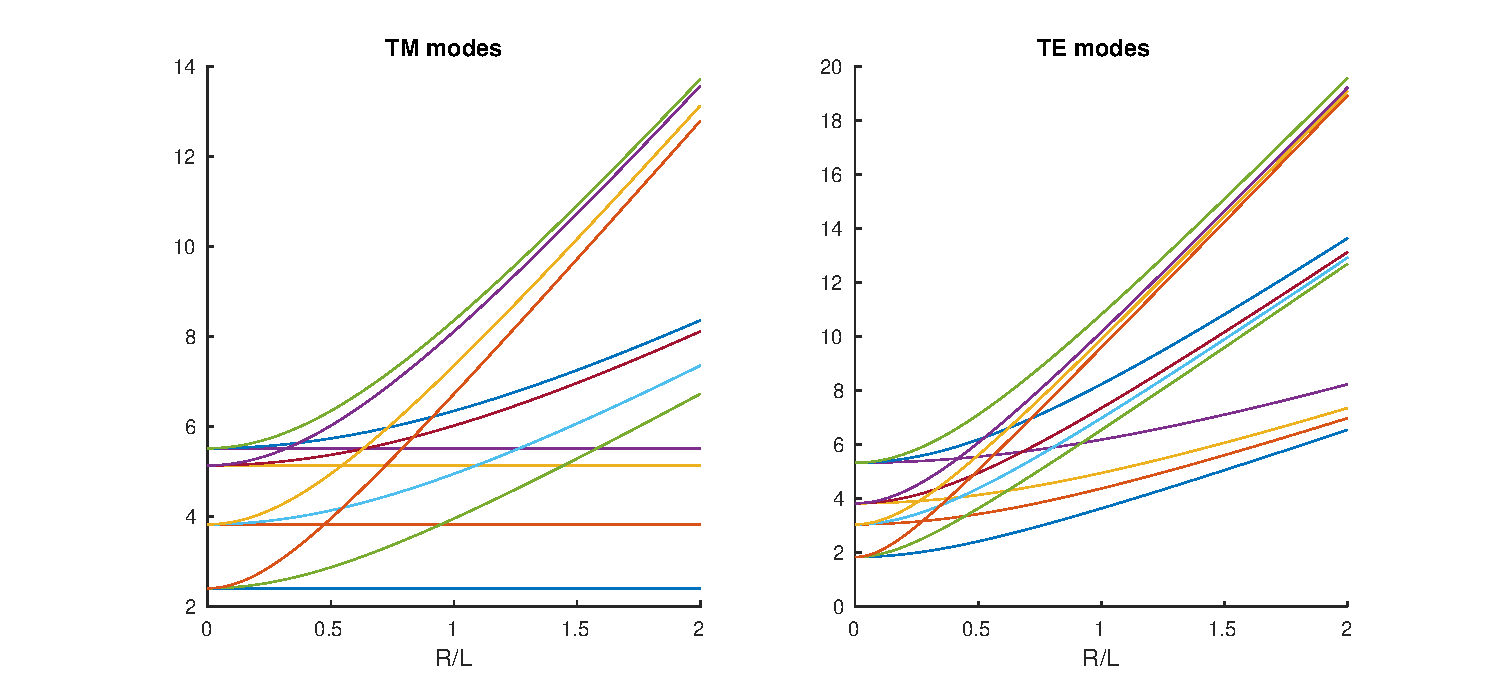
\includegraphics[width=\textwidth]{p8_6}
\end{figure}
\\
b) The lowest mode with $R/L = 2/3$ is the $TM_{01}$ mode.
We find the Q factor from:
\begin{align}
 Q &= \omega \frac{U}{P_{loss}}
\end{align}
For the $TM_{01}$ mode with $p=0$, $U=\frac{L}{2}\int_A |\psi|^2\ da$ from Jackson 8.92.
The power loss is (from Jackson 8.94 taking $\xi = 1$):
\begin{align}
 P_{loss} &= \frac{\epsilon}{2\sigma\delta}\lrp{1+CL/2A}^{-1}\int_A |\psi|^2\ da
\end{align}
Taking the ratio and using the equation for skin depth $\delta = \sqrt{2/\omega\mu\sigma}$:
\begin{align}
 Q &= \frac{L}{\delta}\lrp{1+L/R}^{-1}
\end{align}
For the given dimensions:
\begin{align}
 Q &= \frac{.012}{\delta}
\end{align}
Assuming the interior of the cavity is free space, the fundamental frequency is about $\frac{2.41c}{.02} = 3.61e10$ or about 5.75 GHz.
Pasternack's online skin depth calculator provides a value of $0.860 \mu m$ at this frequency.
Therefore the Q of this cavity is about 14,000.

\section*{9.3}
Since the problem is axially symmetric but not spherically symmetric we expect the dipole term to dominate.
The electric dipole moment is give by:
\begin{align}
 \bv{p} &= \int \bv{x}'\rho(\bv{x}')\ d^3x'
\end{align}
We have previously solved the dipole potential of charged hemispheres:
\begin{align}
 \Phi &= \frac{3}{2}VR^2\frac{1}{r^3}\cos{(\theta)}
\end{align}
The potential from a dipole is:
\begin{align}
 \Phi &= \frac{1}{4\pi\ez}\frac{\bv{p}\cdot \bv{r}}{r^3}
\end{align}
So the dipole moment of the hemispheres is:
\begin{align}
 \bv{p} = 6\pi\ez VR^2\hat{z}
\end{align}
Ignoring the near-field component, we can directly calculate the $\bv{H}$ and $\bv{E}$ fields (Jackson 9.19).
\begin{align}
 \bv{H} &= \frac{ck^2}{4\pi}(\bv{n} \times \bv{p})\frac{e^{ikr}}{r}\\
 \bv{H} &= -\frac{3ck^2\ez}{2}VR^2\frac{e^{ikr}}{r}\sin{(\theta)}\hat{\phi}\\
 \bv{E} &= Z_0\bv{H} \times \bv{n}\\
 \bv{E} &= -\sqrt{\frac{\ez^2\mu_0}{\ez^2\mu_0}}\frac{3}{2}Vk^2R^2\frac{e^{ikr}}{r}\sin{(\theta)}\hat{\theta}\\
 \bv{E} &= -\frac{3}{2}Vk^2R^2\frac{e^{ikr}}{r}\sin{(\theta)}\hat{\theta}
\end{align}
The power radiated per unit solid angle is (Jackson 9.23):
\begin{align}
 \frac{dP}{d\Omega} &= \frac{c^2Z_0}{32\pi^2}k^4|\bv{p}|^2\sin^2{(\theta)}\\
 \frac{dP}{d\Omega} &= \frac{c^2Z_0}{32\pi^2}k^4\lrp{36\pi^2\ez^2V^2R^4}\sin^2{(\theta)}\\
 \frac{dP}{d\Omega} &= \frac{9}{8}c^2Z_0k^4\ez^2V^2R^4\sin^2{(\theta)}
\end{align}
The total radiated power is (Jackson 9.24):
\begin{align}
 P &= \frac{c^2Z_0k^4}{12\pi}|\bv{p}|^2\\
 P &= \frac{3\pi}{Z_0}k^4V^2R^4
\end{align}





\end{document}
